\documentclass[tikz,border=10pt]{standalone}
\usepackage{tikz}
\usetikzlibrary{positioning}
\begin{document}

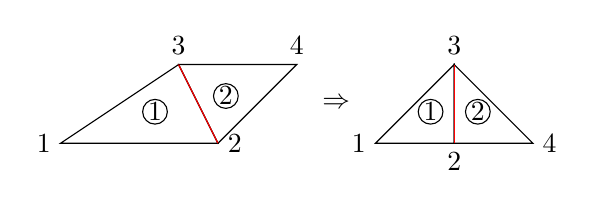
\begin{tikzpicture}[
        scale=1,
        sty/.style={draw,circle,font=\fontsize{10}{10}\selectfont,   inner sep=.1mm}
    ]
    \coordinate [label=left:$1$](A) at (0,0);
    \coordinate [label=right:$2$] (B) at (2,0);
    \coordinate [label=above:$3$] (C) at (1.5,1);
    \coordinate [label=above:$4$] (D) at (3,1);
    \node[sty] at (1.2,0.4){$1$};
    \node[sty] at (2.1,0.6){$2$};
    \draw (A) -- (B)--(C)--cycle;
    \draw (B) -- (C)--(D)--cycle;
    \draw[red](B)--(C);
    \node at (3.5, .5) {$\Rightarrow$};
    \coordinate [label=left:$1$](A) at (4,0);
    \coordinate [label=below:$2$] (B) at (5,0);
    \coordinate [label=above:$3$] (C) at (5,1);
    \coordinate [label=right:$4$] (D) at (6,0);
    \node[sty] at (4.7,0.4){$1$};
    \node[sty] at (5.3,0.4){$2$};
    \draw (A) -- (B)--(C)--cycle;
    \draw (B) -- (C)--(D)--cycle;
    \draw[red](B)--(C);
\end{tikzpicture}

\end{document}
